\documentclass[review]{elsarticle}

\usepackage{lineno,hyperref}
\modulolinenumbers[5]

\journal{Journal of \LaTeX\ Templates}

%%%%%%%%%%%%%%%%%%%%%%%
%% Elsevier bibliography styles
%%%%%%%%%%%%%%%%%%%%%%%
%% To change the style, put a % in front of the second line of the current style and
%% remove the % from the second line of the style you would like to use.
%%%%%%%%%%%%%%%%%%%%%%%

%% Numbered
%\bibliographystyle{model1-num-names}

%% Numbered without titles
%\bibliographystyle{model1a-num-names}

%% Harvard
%\bibliographystyle{model2-names.bst}\biboptions{authoryear}

%% Vancouver numbered
%\usepackage{numcompress}\bibliographystyle{model3-num-names}

%% Vancouver name/year
%\usepackage{numcompress}\bibliographystyle{model4-names}\biboptions{authoryear}

%% APA style
%\bibliographystyle{model5-names}\biboptions{authoryear}

%% AMA style
%\usepackage{numcompress}\bibliographystyle{model6-num-names}

%% `Elsevier LaTeX' style
\bibliographystyle{elsarticle-num}
%%%%%%%%%%%%%%%%%%%%%%%

\begin{document}

\begin{frontmatter}

\title{The state of big data reference architectures: a systematic literature review}

%% Group authors per affiliation:
% \author{Elsevier\fnref{myfootnote}}
% \address{Radarweg 29, Amsterdam}
% \fntext[myfootnote]{Since 1880.}

%% or include affiliations in footnotes:
% \author[mymainaddress,mysecondaryaddress]{Elsevier Inc}
% \ead[url]{www.elsevier.com}

% \author[mysecondaryaddress]{Global Customer Service\corref{mycorrespondingauthor}}
% \cortext[mycorrespondingauthor]{Corresponding author}
% \ead{support@elsevier.com}

% \address[mymainaddress]{1600 John F Kennedy Boulevard, Philadelphia}
% \address[mysecondaryaddress]{360 Park Avenue South, New York}

\begin{abstract}
This template helps you to create a properly formatted \LaTeX\ manuscript.
\end{abstract}

\begin{keyword}
\texttt{elsarticle.cls}\sep \LaTeX\sep Elsevier \sep template
\MSC[2010] 00-01\sep  99-00 s
\end{keyword}

\end{frontmatter}

\linenumbers

\section{Introduction}

The rapid development of software technologies, the proliferation of digital devices and networking infrastructure of today, have by and large, augmented user’s capability to generate data \cite{AtaeiSecurity}. In the age of information, users are unceasing generators of structured, semi-structured, and unstructured data that if collected and crunched correctly, may reveal game-changing patterns \cite{AtaeiACIS}.

The unprecedented proliferation of data have emerged a new ecosystem of technologies; one of these ecosystems is big data (BD)\cite{AtaeiHype}. BD is a term emerged to describe large amount of data that comes in various forms from different channels. Within the years, BD has attained a lot of attention from academia and industry, and many strive to benefit from this new material. Howbeit, adopting BD requires the absorption of great deal of complexity and many traditional systems cannot cope with characteristics of this domain. 

A recent survey published by Databricks in partnership with MIT Technology Review Insights, stated that only 13\% of companies excel at delivering on their data strategy \cite{DataBricks}. In the same vein, Vintage Partners highlighted that only 24\% of companies have successfully adopted BD \cite{NewVantageSurvey}. Sigma computing report presented that 1 in 4 business experts have given up on getting insights they needed because the data processing took too long \cite{SigmaSurvey}. Moreover, Gartner approximated that only 20\% of companies have successfully adopted BD. 

Some of the most highlighted challenges of BD is 'lack of business context', 'organizational challenges', 'BD architecture', 'data engineering', 'rapid technology change', and 'lack of talent' \cite{AtaeiBigDataEnvirons}. Whereas similar issues may exist in other domains, it is exacerbated when it comes to BD systems. This is due the inherent complexity of BD engineering, the need for real-time processing, the scalability requirement of these systems, and the sensitivities around data.

Today, majority of BD systems are designed underlying ad-hoc and complicated architectural solutions \cite{Gorton}, that do not seem to adhere to similar patterns. This will challenge software architects to design a suitable solution for any given context, creates a foundation for an immature architectural decision, and does not promote the growth and development of BD systems as a whole. 

Therefore, since the approach of ad-hoc design to BD systems is undesirable and leaves many engineers in the dark, there is a need for more software engineering research for BD systems. To this end, this study presents a systematic literature review (SLR) on BD (BD) reference architectures (RAs). 

\section{Why reference architectures?}
Conceptualization of the system as an RA, helps with understanding of the system’s key components, behavior, composition and evolution of it, which in turn affect quality attributes such as maintainability, scalability and performance \cite{Cloutier}. Therefore RAs can be a good standardization artefact and a communication medium that not only results in concrete architectures for BD systems, but also provide stakeholders with unified elements and symbols to discuss and progress BD projects.

This approach to system development is not new to practitioners of complex system. In software product line (SPL) development, RAs are utilized as generic artifacts that are instantiated and configured for a particular domain of systems \cite{Derras}. In software engineering, IT giants like IBM have referred to RAs as the 'best of best practices' to address complex and unique system design challenges \cite{Cloutier}. In other international standardization, RAs have been repeatedly used to standardize an emerging domain, a good example of this is BS ISO/IEC 18384-1 RA for service oriented architectures \cite{Iso18384-1}. 

\section{State of the art}

Despite the undeniable benefits of RAs, and their potential to solve some of the complex issues of BD systems, we think that this area is underdeveloped and needs more attention from both academia and practice. This insight is derived from our preliminary systematic review in academia, and a search for available big data RAs (\cite{AtaeiACIS}).

To the best of our knowledge, one of the most comprehensive BD RA published, is the National Institute of Standards and Technology (NIST) BD RA. This RA is published by Big Data Public Working Group (NBD-PWG) with large set of contributors from academia, industry, non-profit organizations, agents, and government representatives. This was announced as an initiative from White house in March 2012, and the the RA was published under the title 'NIST Big Data Interoperability Framework: Volume 6, Reference Architecture' in October 2019. 

Given the substantial investment on BD RAs, one might infer the value of these artifacts, and this can in turn highlights the necessity for more research in this domain. Another factor that worths mentioning is how vaguely the phrase 'reference architecture' is defined and institutionalized. For instance, the difference between a 'concrete architecture' and an RA is hardly discussed, and different domains seem to have defined the artifact slightly differently. For instance, Cloutier et al (\cite{Cloutier}) defined RAs as 'Reference Architectures capture the essence of existing architectures, and the vision of future needs and evolution to provide guidance to assist in developing new system architectures'. This definition is derived from the system engineering domain and by the means of collaborative forum from Steven's institute of technology. 

In another effort, Muller et al (\cite{muller2008reference}) defines RA as 'artifacts that captures the essence of architecture of a collection of systems. This definition is driven from the product line engineering domain'. Moreover, the difference between RAs and concrete architectures is rarely discussed. Another definition by Bass et al (\cite{Bass}) stated that 'A reference architecture is a reference model mapped onto software elements (that cooperatively implement the functionality defined in the reference model) and the data flows between them'. 

Angelov et al (\cite{angelov2009classification}) defined RAs proposed that 'A reference architecture is a generic architecture for a class of information systems that is used as a foundation for the design of concrete architectures from this class'. Although different authors may have defined RAs with different syntax, the essence remains the same: to reuse the software engineering knowledge for a class of systems, particularly in relation to architecture. 

Given the failure rate of BD projects, we posit RAs as potential solution to facilitate system development and BD architecture, and aim to explore this area through a systematic literature review. Up to date, there's only one SLR that explored this area (\cite{AtaeiACIS}), which is outdated, suffers from methodological clarity, and is published as a conference paper, which implies lack of detail.

Based on this, the objective of this review is to find and collate the BD RAs available from the body of evidence, highlight their architectural commonality and point out the limitations. This study can be considered a useful primer for practitioners or academics who are interested in partaking in a BD project. 

The research questions are formulated as the following; 
\begin{enumerate}
    \item What are current BD RAs available in academia and industry?
    \item What are major architectural components of these BD RAs? 
    \item What are the limitations of current BD RAs?
\end{enumerate}


\section{Review Methodology:}
This research follows the guidelines of PRISMA (\cite{page2021prisma}). In addition, we adopted PRISMA-S (\cite{rethlefsen2021prisma}) to improve our search strategy and lastly we have used Barbara et al's guidelines for evidence based software engineering and systematic reviews \cite{kitchenham2015evidence}. Although PRISMA is a comprehensive guidelines on conducting a systematic literature review, it is derived from the healthcare community and sometimes makes assumptions that may not be relevant to software engineering and information system researchers. Barbara et al \cite{kitchenham2015evidence} has translated many of these assumptions to the domain of software engineering and included many guidelines for lone researchers and projects with small number of researchers. 

We have therefore utilized PRISMA as the underpinning of our research design, with complementary studies to reduce bias, improve transparency and systematiticity. SLR has been chosen because it is a qualitative research methodology that is aimed at driving knowledge and understanding about the subject matter and the elements surrounding it. Besides, SLR provides a transparent and reproducible procedure that elicits patterns, relationships, trends, and delineates the overall picture of the subject \cite{borrego2014systematic}.

The main objective of this study is to assess the current state of BD RAs, identify their major architectural components, point out fundamental concepts and discuss their limitations. This objective is achieved in four phases. In first phase, research questions are stated, literature are identified and pooled, exclusion and inclusion criteria are defined, and the quality framework is developed. In second phase, the title of the studies are assessed based on the inclusion and exclusion criteria. After that, the filtered studies are once more assessed based on their title, abstract, introduction and conclusion. After this, full analysis of the studies took place by running each study against the criteria defined in the quality framework. Thirdly, selected pool of literature is coded based on research questions. Lastly, findings are synthesized by the means of thematic synthesis, and themes realized are depicted.

This study builds on the SLR conducted by Ataei et al \cite{AtaeiACIS} and aims to improve it by covering the years 2020 to 2022. Unlike Ataei's work, this paper aims to employ thematic synthesis, and provide a more detailed view of BD RAs and their properties.

\subsection{Identification}

The first phase of the SLR began, by adoption of PRISMA-S (\cite{rethlefsen2021prisma}) to develop a robust multi-database search strategy. This extension of PRISMA provided us with a framework of 12 items to increase transparency, systematiticity, and reduce bias. For the purposes of this study, following electronic databases were search: ScienceDirect, IEEE Explore, SpringerLink, AISeL, JSTOR and ACM library. To pursue to goal of finding all literature available on the topic, and to avoid overlooking valuable research, abstract and citation databases and search engines such as Google Scholar, and Research Gate was used.

We also searched the grey literature on the topic, using the search string "big data" AND "reference architecture*" on Google ( in June 2022 ). The first 40 results were selected for screening. This was done in 'incognito mode' to avoid any personal customization of the google search pages. Reference lists of included studies were manually screened to identify additional studies. This is to achieve the critical component of 'completeness' as suggested by Kitchenham et al \cite{kitchenham2015evidence}.

The platform search capabilities varied, but our search strategy remained uniform for most parts. For instance, if a platform did not support wildcards ( like asterisk ), we just searched twice for the singular and plural version of the word. The only exception that made the selection process longer was SpringerLink, because it did not support bulk download of references in BibTex format. The reproducible search for the chosen databases is as follows: 

\begin{itemize}
    \item ("Document Title":big data) AND ("Document Title":reference architecture) OR ("Document Title":big data architecture)
\end{itemize}

The reason we included architecture is due to the fact that terms \emph{reference architecture} and \emph{architecture} may have been used interchangeably, and an architecture that is at the abstraction level of an RA, might have been called just an architecture. Therefore it was critical for us to firmly define these terms and then categorize studies based on these definitions. These definitions and our findings are depicted in the findings section.

Our initial search was set to year 2020 to year 2022, as the work of Ataei et al \cite{AtaeiACIS} covered the years 2010-2020. Nevertheless, we still included the years 2010 to 2020 to make sure no research is left out or overlooked. These years are chosen firstly because more contemporary researches are focused on the facilitation of big data system development, and secondly there's no SLR that has covered those.

It is worth mentioning that what we refer to by \textit{limit} here should, not be confused with \textit{filters} or inclusion criteria. To achieve these limits, we have utilized databases features. All databases supported the selection of year range, and the language limit was automatically applied by doing an advanced search with the aforementioned keywords.

Our approach to systematic collection of evidence was to search databases using the keywords aforementioned and then bulk download the BibTex files. Majority of the databases supported bulk downloading of BibTex files except for SpringerLink, Google Scholar, and Research Gate. For SpringerLink we downloaded the studies in CSV format and then converted them to a BibTex using a custom script. For Google Scholar and ResearchGate, unfortunately, we had to take the manual path of creating a bib file for the studies. 

Once all the bib files have been created, we merged them into one large bib file and imported it to a software called JabRef (\cite{JabRef}) for deduplication. 172 studies are pooled initially, out of which 6 duplicates have been identified. We removed the SLR that this study is based on, and also another paper that we could not find the citation for. In the other hand, we found 5 white papers and 4 website blogs and added them to the selection pool. At the end of this phase, 173 studies have been pooled. 

\subsection{Screening and Eligibility}

Stage 1 of screening started with assessing the title, abstract, and keywords of the pooled studies. For grey literatures simply the title. This was achieved based on our inclusion and exclusion criteria; 

\begin{itemize}
    \item Primary and secondary studies (including grey literature) between Jan 1st 2010 and June 1st 2022 on the topics of BD RAs, BD models, and BD architectural components were included. 
    \item Research that Indicates the current state of RAs in the field of BD and demonstrates possible outcomes
    \item Studies that are scholarly publications, book, book chapter, thesis, dissertation, or conference proceedings 
    \item Grey literature such as white paper that includes extensive information on BD RAs
\end{itemize}

And the studies with the following topics were excluded: 

\begin{itemize}
    \item Informal literature surveys without any clearly defined research questions or research process
    \item Duplicate reports of the same study (a conference and journal version of the same paper)
    \item Short papers (less than 5 pages)
    \item Studies that are not written in English
\end{itemize}

Disagreement among researchers were resolved using Krippendorff’s alpha (\cite{krippendorff2011computing}). Our aim was not to get involved in a very complicated statistics model, so we've done most of the computations using SPSS, specifically with Hayes’ Macro. We made sure that a separate file is created for each variable, and inserted coders as variables and not a constant value. Our \begin{equation} \alpha \end{equation} value was within the acceptable range (above 80), and any disagreement was solved by inviting a third person or a moderator. When \begin{equation} \alpha \end{equation} value was very low (indicating a low reliability), we stopped the process, and tried to clarify fundamental concepts and categories. The final computed \begin{equation} \alpha \end{equation} value was 89.9\%. 

In stage 2, After excluding papers based on inclusion and exclusion criteria, and as suggested by Kitchenham et al \cite{kitchenham2015evidence}, we assessed studies based on their quality. Quality of the evidence collected as a result of this SLR has direct impact on the quality of the findings, making quality assessment an important undertaking. Therefore it is imperative for us to realize how much confidence we can place in the conclusions and findings arising from the evidence collected to form a great whole, that is themes and models in this case. 

However, this process comes with some well-known complexities. The most fundamental ones are perhaps firstly defining the term 'quality', and secondly trying to appraise the quality of conference papers that rarely provide enough detail on research methodology and evaluation. Generally, a quality of a study is tightly associated to its research method and the validity of its findings. From this perspective, and inspired by the works of Noblit and Hare on meta-ethnography (\cite{noblit1988meta}), and Dyba et al (\cite{dybaa2008empirical}), quality of studies is assessed by the extent to which the conduct, design and analysis of a research is susceptible to systematic errors or bias (\cite{cumpston2019updated}). That is, the more bias in the selected literature, the more chance to create miss-leading conclusions.

Considering the rather heterogeneous nature of software engineering and information systems (IS) papers, and difficulty of defining quality in studies with varying nature, we first analyzed a few well-established checklists such as Critical Appraisal Skills Programme (CASP \cite{CASP}), and JBI's critical appraisal tool (\cite{JBI}). Whereas these checklists could potentially account for the requirements of this study, we opted for something that is more specific to software engineering and IS. We realized for example that, Runeson et al (\cite{runeson2006we}) provided a checklist designated to help researchers reading and undertaking software engineering case studies. In the same vein, Dyba et al (\cite{dybaa2008empirical}) proposed a quality criteria based on CASP checklist for qualitative studies in software engineering systematic reviews. 

Nevertheless, the challenge is that our study includes a large number of different study types that needs to go through a single checklist. To address this, we developed a criteria made up of 11 elements. These criteria are informed by those proposed by CASP for assessing the quality of qualitative research (\cite{CASP}) and by guidelines provided by Kitchenham (\cite{kitchenham2002preliminary}) on empirical research in software engineering. The 7 criteria tested literature on 4 major areas that can critically affect the quality of the studies. These categories and the corresponding criteria are as following;

\begin{enumerate}
    \item \emph{Minimum quality threshold:} 
    \begin{enumerate}
        \item Does the study report empirical research or is it merely a 'lesson learnt' report based on expert opinion ?
        \item The objectives and aims of the study is clearly communicated, including the reasoning for why the study was undertaken ? 
        \item Does the study provide with adequate information regarding the context in which the research was carried out ?
    \end{enumerate}
    \item \emph{Rigour:}
    \begin{enumerate}
        \item Is the research design appropriate to address the objectives of the research ?
        \item Is there any data collection method used and is it appropriate ?
    \end{enumerate}
    \item \emph{Credibility:}
      \begin{enumerate}
        \item Does the study report findings in a clear and unbiased manner ? 
     \end{enumerate}
    \item \emph{Relevance:}
    \begin{enumerate}
        \item Does the study provides value for practice or research 
     \end{enumerate}
\end{enumerate}

Taken all together, these 7 criteria gave us a measure of the extent to which a particular study's findings could make a valuable contribution to the review. These criteria was disseminated as a checklist among researchers with value for each property being dichotomous, that is 'yes' or 'no' in two phases. In the first phase, researchers only assess the quality based on the first major area ( minimum quality threshold ). If the study passed the first phase, it would then go into the second phase, where it was assessed for credibility, rigour and relevance. The quality is agreed if 75\% of the responses are positive for any given study with at least 75\% inter-rater reliability. 

Disagreements regarding the quality was usually resolved through a meeting. While, the meeting could not address the disagreements, a moderator has been invited to the process. Lastly, it is worth mentioning that this quality framework was not used for grey literature. Grey literature were only assessed through inclusion and exclusion criteria. 

In the first phase (identification) of this SLR, a total of 138 literature has been pooled from academia, and 24 from grey literature. Some of this literature has been added to the pool by the process of forward and backward searching. For instance, by reading NIST RA, we found out about Oracle, Facebook, and Amazon RAs and included those in the pool of the literature as well. 

In the screening phase, the literature that were not in-line with our inclusion and exclusion criteria have been eliminated. For example, if the paper was very short and was not on the topic of BD RA, or its ecosystem or limitations, it was excluded. As a result of this phase, 50 papers excluded. In the next phase, by assessing studies against the quality framework, 21 studies from academia, and 12 studies from grey literature pool has been eliminated. 

At the end of the selection and screening process, 79 papers have been pooled. The detail of this process is depicted in \ref{fig:PRISMA}.

\begin{figure}[t]
    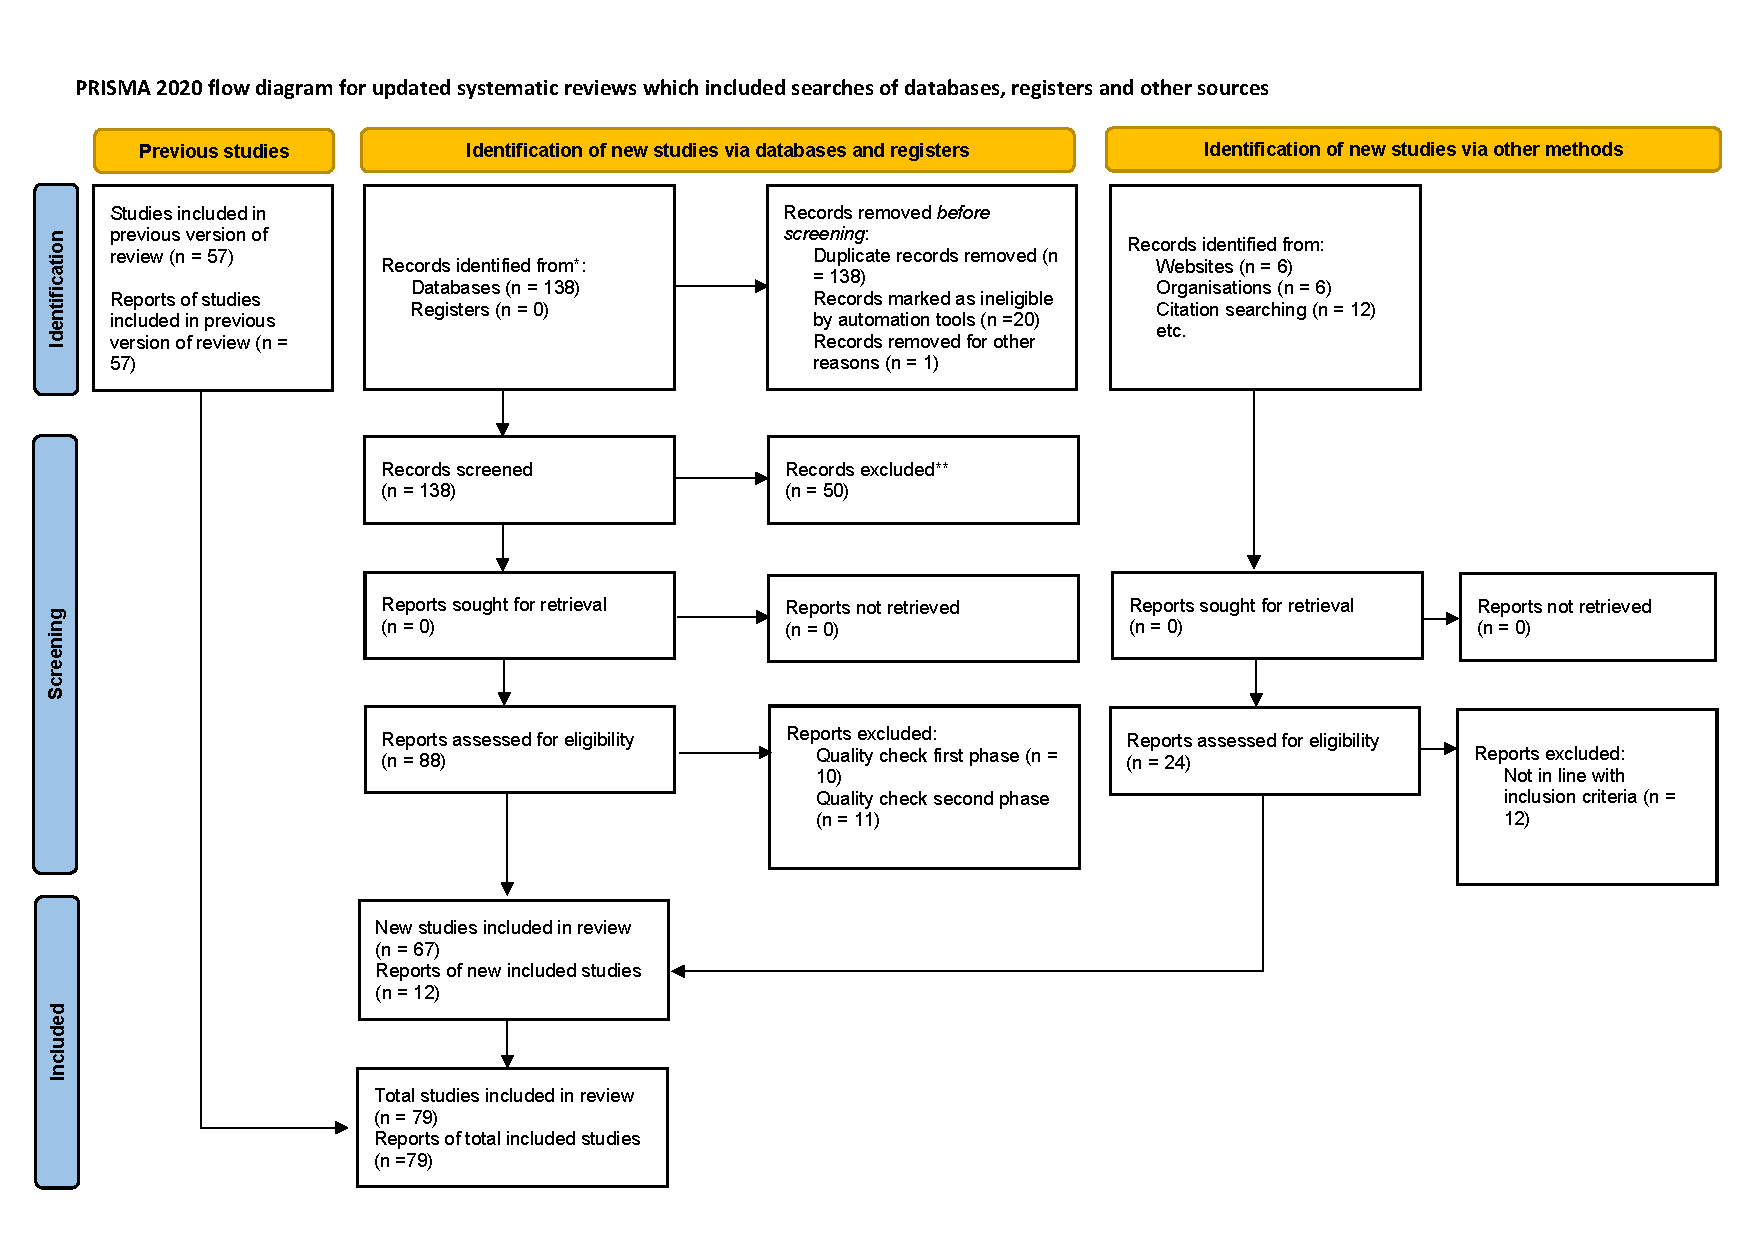
\includegraphics[width=13cm]{PRISMA/PRISMA_Flow_Diagram.pdf}
    \caption{PRISMA flowchart}
    \label{fig:PRISMA}
\end{figure}

By the result of this work, 79 articles have been selected comprising of proceedings, journal articles, book chapters, and white papers. Out of the pool of articles, 33.3\% are from IEEE Explore, 5.2\% from ScienceDirect, 24.5\% from SpringerLink, 15.7\% from ACM, and 21\% from other sources such as Google Scholar and Research Gate. 30 journal articles, 29 conference proceedings, 12 book chapters, 6 white papers, 1 Master’s Thesis and 1 PhD thesis were selected. 55\% of the articles were selected from the years 2016- 2022, 33\% belonged to years 2013-2016, and the rest to years 2010-2013. These stats are portrayed in \ref{fig:SLRStats}

\begin{figure}[t]
    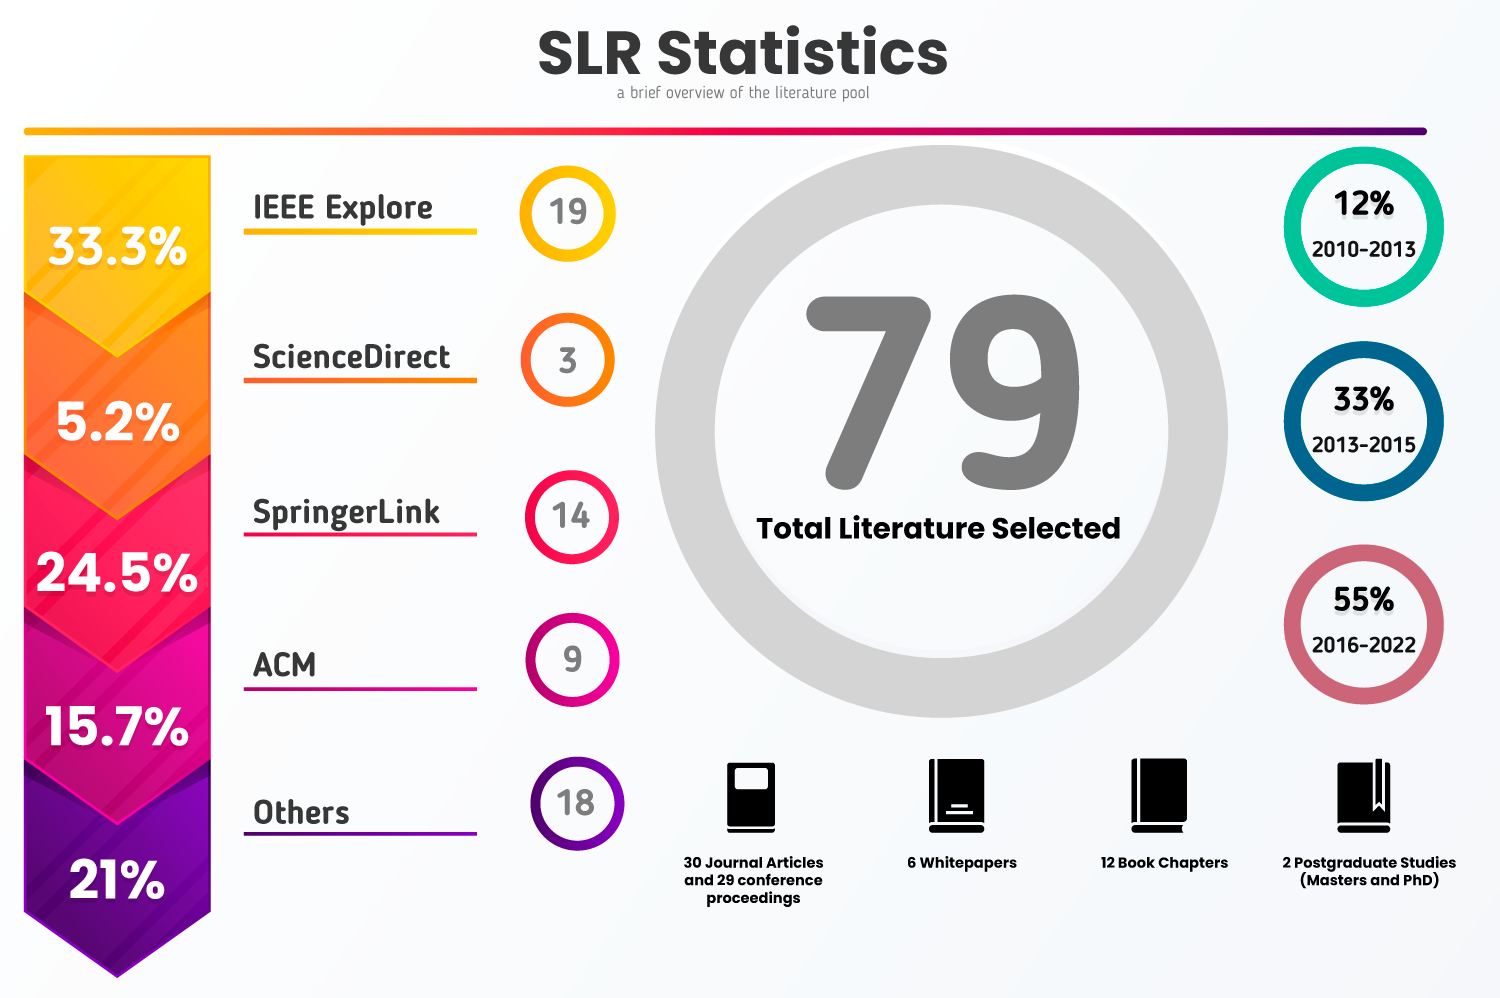
\includegraphics[width=13cm]{Media/databases-statitistic-[Recovered].png}
    \caption{SLR Statistics}
    \label{fig:SLRStats}
\end{figure}

\subsection{Data Extraction and Synthesis}

By this stage, research questions have been set, inclusion and exclusion criteria are defined and applied, the quality assessment framework is developed and applied to the pool of studies, and the research embarked on actual synthesis of data. An integral element of this phase is data extraction, in which the essence of the studies are obtained in an explicit and consistent manner.

Precursor to synthesis of the actual data, we first followed the guidelines proposed by \cite{cruzes2011recommended} for data extraction. Data extraction firstly began by reading the entire pool of literature in order to get immersed with the data \cite{braun2006using}. From there on, we followed a structured reading approach and extracted three kind of data; 1) Publication Details (author, title, year, etc), 2) Contextual descriptions ( industry, settings, technologies ), and 3) Findings ( results, the actual RA, events, etc ..)

Through process was a bit challenging, as some studies did not describe the method adequately, contextual information were not detailed often, and evaluation methods varied. To overcome this challenge, majority of this process took place in a consensus meeting \cite{dyba2007applying}.

After data extraction, we began the coding process. For this step, we've had several approaches ahead of us. Either we could adopt a deductive or a prior approach (\cite{miles1994qualitative}) or an inductive or Grounded Theory approach (\cite{corbin2014basics}). Neither of which could be as rigorous as we desired, thus we opted for an integrated approach (\cite{lofland1971analyzing}). We used the software Nvivo to organize our files and created an initial set of a priori codes based on research questions. These codes are as followings;

\begin{enumerate}
    \item BD RAs (RQ1)
    \item BD RAs Architectural components (RQ2)
    \item BD RAs limitations (RQ3)
\end{enumerate}

As the coding progressed, we realized that there is a need to define some of the fundamental areas that seem to not have been well established in academia and practice. For instance, we've been looking for a comprehensive data to discuss the fundamental concepts of RA to further support our initiative, but this was not standardized, and while there was mention of these concepts, they were usually lacking or very short. Furthermore, not many studies discussed the benefits and relevance of RAs for BD systems. We also could not find a study that thoroughly discusses common approaches to developing BD RAs, and the challenges of developing a BD RA.

Based on these, therefore, we added the following extra four codes;
\begin{enumerate}
    \item Fundamental concepts of RAs
    \item How can RAs help BD system development
    \item Common approaches to creating BD RAs
    \item Challenges of creating BD RAs
\end{enumerate}


% Most literature selected were within the years 2016-2021 as they provided with most recent and relevant information. Howbeit, some studies dating back to 2010 have been included to provide fundamental knowledge regarding big data systems, reference architectures and architecture evaluation.

% After the initial search, it becomes apparent that AISeL and Elsevier are good sources for good quality big data literature, whereas MIS Quarterly provided with the highest quality of Information Systems (IS) research.

\section{Improvements}

\begin{enumerate}
    \item The current writing style looks like a summary description, lacks new insight on the topic. The overall contribution needs to be enhanced.
    \item In general, each larger-scale system requires a more understanding of architectural components, owing largely to the complex nature of system architects. However, I cannot find a case that the authors demonstrate the uniqueness of BD systems, and the actual development challenges in BD systems.
    \item The findings yielded by investigating the research questions of this SLR should constitute many discussion points around the research and practice of BD systems. However, the manuscript is completely missing a discussion section. One should expect that the results of SLR can inform the current knowledge and provide several research directions for future research. 
    \item Last, one of the core challenges with the paper is to situate it within an ongoing scholarly conversation. The authors currently reference a fairly diverse set of papers, but remain at a fairly abstract level when it comes to elaborating how your work builds upon and expands existing work. In turn, this makes it difficult to appreciate theoretical implications of your work. 
\end{enumerate}
 

\bibliography{mybibfile}

\end{document}